\documentclass{whutmod}
\usepackage{metalogo}
\usepackage{float}
\usepackage{subfigure} 
\usepackage{url}
\usepackage{booktabs}
\bibliographystyle{unsrt}
\team{23}
\membera{刘子川}
\joba{编程}
\memberb{程宇}
\jobb{建模}
\memberc{陈荣兴}
\jobc{建模}
\hypersetup{
	colorlinks=true,
	linkcolor=black
}

\title{基于因子分析与灰色关联分析对武汉市人才吸引力的量化评价}
\tihao{4} 

\begin{document}


	
	\begin{abstract}



本文基于多背包优化模型,设计\textbf{沙石算法},优化部队的装载方案。再通过\textbf{遗传算法}与\textbf{泊口仿真模型},选择出装载方案中装载时间最少,需要船支数量最少的装载方案。最后在\textbf{泊口仿真模型}中添加港口摧毁事件,再次使用使用遗传算法求解出港口被摧毁对应的最佳装载方案。
~\\

针对问题一,将原问题转化成多背包优化问题,设计\textbf{沙石算法},优化部队装载方案。根据题目要求,首先对兵力、装备与船载的面积进行量化,得到相关的有效面积值。然后建立船舰数量的决策向量,以调用船支数量作为目标函数,题中船舰装载限制作为约束条件,建立\textbf{部队装载优化模型}。设计\textbf{沙石算法},进行装备均分和部队装载,求解得到各旅级单位装备人口的装载方案和各类舰船的使用数量。各类船舰的有效面积利用率基本达到$\textbf{90\%}$以上,共使用船舰数\textbf{236艘}。
~\\



针对问题二,调整问题一中的\textbf{沙石算法}作为验证算法,并搭建\textbf{泊口仿真模型}计算每种装载方案需要的装载时间作为适应度函数,代入\textbf{遗传算法}求得最佳装载方案。本组首先基于问题一中设计的\textbf{沙石算法},编译验证算法,以验证每种装载方案是否能装载全体部队。然后设计\textbf{泊口仿真模型},使每个港口以最大工作效率工作,计算用时最长泊口装载所用时间作为总装载时间。再利用遗传算法,将每种民用船调用量作为染色体,搜素总装载时间最少,使用总船支数量最少的调用方案。最优方案为军用登陆舰\textbf{全部调用},民用船调用方案为2万吨级滚装船\textbf{15艘},3万吨级滚装船\textbf{5艘},集装箱船\textbf{1艘},杂货船\textbf{1艘}和客船\textbf{1艘}。装载时间为\textbf{20小时},共使用船舰\textbf{364艘}。
~\\

针对问题三,基于问题二中的模型,延用遗传算法,并调整\textbf{泊口仿真模型},增加摧毁泊口事件,求解出泊口被摧毁对应的最佳装载方案。首先调整\textbf{泊口仿真模型},当运行时间等于攻击时间时,停止被摧毁港口正在进行的任务,并将任务进度清零,并在之后的检索列表中剔除被摧毁泊口。重新运行遗传算法以寻找港口被摧毁对应的最佳装载方案。最优方案为军用登陆舰\textbf{全部调用},民用船调用方案为2万吨级滚装船\textbf{18艘},3万吨级滚装船\textbf{3艘},集装箱船\textbf{1艘},杂货船\textbf{1艘}和客船\textbf{1艘}。装载时间为\textbf{20小时},共使用船舰\textbf{365艘}。
~\\

本文中所提到的模型优点主要有两点:一、使用沙石算法与泊口仿真模型,使得军舰与泊口的利用率达到较高水平,最终方案转载时间少,使用船支数量少;二、利用遗传算法优化装载方案,鲁棒性强,全局搜素能力强。

	
  
\keywords{沙石算法\quad  遗传算法\quad  泊口仿真模型\quad 部队装载优化模型\quad }



	\end{abstract}
	
	%目录
	\tableofcontents
	\newpage	%换页符
	
	\section{问题重述}	
	\subsection{问题背景}
    随着全球化的进程,人类活动范围日益扩大,人群流动频繁,传染病可在大范围内迅速传播,是对人类社会存在威胁的公共卫生问题。在疾病控制实际工作中,疾病的发病与流行趋势分析是极其重要的一环,科学、准确的分析能对卫生行政部分制定疾病预防与控制策略产生重要的影响,传染病早期预警将大大降低传染病的社会经济危害。
    
    为了提高某传染病疫情和突发公共卫生事件报告的质量和时效,加强对全国感染病人的诊断、治疗和督导管理,卫生部建立了全国监管机制,及时通报相关病情和相关数据,并通过对疫情数据的动态分析,建立该传染病防治工作督导检查、防治效果评价和制定防治对策和策略,控制并逐渐消灭该传染病。构建预测模型从早期探测到传染病的爆发并及时预警,采取应对措施,是目前传染病防控的重要手段,具有重要的实际意义。
    
    

	\subsection{问题概述}
    围绕相关附件和条件要求,研究海运装载行动输送兵力任务的合理安排,依次提出以下问题:
		 
	
	\textbf{问题一:}根据合适的指标建立模型,分析流行病在2004-2016年的变化趋势,并预测2019年全国感染该病的发病数和死亡数。
	
	\textbf{问题二:}基于2004-2016年每隔三年的不同地区的和职业分类的数据,建立疾病传播模型,并预测2019年传染病重点防控前3名的区域和职业人群。
		
	\textbf{问题三:}结合地区经济发展的相关数据,选择一个角度建立传染病与经济发展相关的模型,并分析结论。
	
	\textbf{问题四: }综合模型结果及分析,给卫生健康委员会相关部门写一封公开信,谈谈对传染病疫情防治的看法和建议。
	
	
	\section{模型假设}
	\begin{itemize}                                             
		\item [(1)] 为保证预测结果精确性,假设题目所给出数据真实可信。
		\item [(2)] 为了优化运算结果,假设所有全副武装的士兵都保持坐姿休息。
		\item [(3)] 假设在战争中,装载消耗更少时间的优先度高于使用更少的民用船。
		\item [(4)] 假设在装载过程中,同一泊口的船舰装载交替时间可以忽略不记。
		\item [(5)] 假设港口被摧毁时,由于提前得到信息,港口上的船只与兵力没有损失,只是正在进行的装载工作停止,且进度完全损失。
	\end{itemize}
	
	
	\section{符号说明}
	\begin{table}[H]
	\label{biao} \centering

	\begin{tabular}{cc}
		\toprule[1.5pt]
		\multicolumn{1}{m{5cm}}{\centering 符号} & \multicolumn{1}{m{5cm}}{\centering 说明} \\
		\midrule[1pt]		
		$X_{i}$  &  第i型装备 \\ 
		$s_{xi}$  &  装备$X_{i}$的占用面积 \\ 
		$l_{i}$  & 装备$X_{i}$的长\\
		$w_{i}$  &  装备$X_{i}$的宽 \\ 
		$\varepsilon _{i}$ & 装备$X_{i}$的面积修正系数\\
		$p_{i}$	 &  全副武装人员数  \\ 
		$eta_{1}$ &  海军船舰的有效面积率 \\ 
		$eta_{2}$	 &  民用船只的有效面积率 \\ 
		$y_{k}$  &   登陆舰数量\\ 
		$z_{n}$  &  民用船数量\\	
		$D$ & 决策向量\\
		$S_{D}$ &  舰载面积系数向量\\ 
		$S_{z}$ & 民用船有效面积向量\\
		$S_{y}$ & 登陆舰有效面积向量\\
		$S_{p}$ & 每营人口面积向量\\
		$A^{k}$  & 面积规划向量\\
		$T_{n}$ & 颖编制总部对数列\\
		$P_{n}$ & 船舰面积数列\\
		$\eta $ &  平均有效面积利用率\\

		\bottomrule[1.5pt]
	\end{tabular}
\end{table}

	\section{问题一模型的建立与求解}
    \subsection{问题描述与分析}

<<<<<<< HEAD
    问题一要求,根据附件中2004年至2016年的流行病相关数据,预测2019年全国感染该疾病的发病人数和死亡人数。本组首先选择合适的指标后建立\textbf{灰色预测}模型,预测分析2004-2019年该流行病的发病人数和死亡人数。再通过\textbf{马尔科夫模型},由2004-2016年的数据模拟残差在各个区间的分布,计算2017-2019年预测残差的期望值。最后将预测结果与残差期望做差,\textbf{校正}传统灰色预测的固有偏差,经过两种模型的有效结合达到科学预流行病的未来发展趋势。其问题一思维流程图如图~\ref{lct}~所示:
       \begin{figure}[H]
   	\centering
   	
\includegraphics[width=\textwidth]{figures/lctc.png}
   	\caption{问题一思维流程图}\label{lct}
   \end{figure}

   
	    \subsection{模型的建立}
	    \subsubsection{灰度预测GM(1,1)}
	    设2004-2016年总发病人数为时间序列:
	     \begin{gather*}
	    X^{(0)}=[x^{(0)}(1),x^{(0)}(2),\cdots,x^{(0)}(13)]
	    \end{gather*}
	    
	    通过一次累加生成1-AGO序列:
	    \begin{gather*}
	    X^{(1)}=[x^{(1)}(1),x^{(1)}(2),\cdots,x^{(1)}(13)]
	    \end{gather*}
	    式中:$x^{(1)}(k)=\sum_{i=1}^{k}x^{(1)}(i),k=1,2,\cdots,13$。
	    
	    根据1-AGO序列建立微分方程为\cite{bib:one}:
	     \begin{gather}\label{333}
	    \frac{d X^{(1)}}{dt}+a X^{(1)} = u
	     \end{gather}
	     式中:$a$称为发展灰度,$u$称为内生控制灰度。设$\widehat{\alpha }$为待估参数向量,且$\widehat{\alpha }=[a,u]^T$,利用最小二乘法求出:
	     \begin{gather}
	     \widehat{\alpha }=(B^TB)^{-1}B^{T}Y_{n}
	     \end{gather}
	     
	     求解方程(~\ref{333}~),可得第$k+1$年传染病发病数\textbf{初步预测模型}为:
	     \begin{gather}
	     \widehat{X}(k+1)=[X^{(0)}(1)-\frac{u}{a}]e^{-ak}+\frac{u}{a},k=1,2,\cdots,16
	     \end{gather}
	     
	     同理将死亡数作为向量$X^{(0)}=[x^{(0)}(1),x^{(0)}(2),\cdots,x^{(0)}(13)]$带入模型可求得2017-2019年死亡数灰度预测值。
	     \subsubsection{马尔科夫模型校正}
	     利用马尔科夫模型对GM(1,1)预测误差项的状态及状态概率进行预估,并利用预测状态的期望值对GM(1,1)预测值进行修正\cite{bib:2}。用2004-2016年预测数据与真实数据残差进行状态划分,设残差序列为:
	     \begin{gather*}
	    \varepsilon =[\varepsilon(1) ,\varepsilon(2), \cdots,\varepsilon(13)]
	     \end{gather*}
	     
	    最大残差绝对值为$\delta _{max}=\underset{1\leqslant i\leqslant13 }{max}\left | \varepsilon(i) \right |$,将预测误差化均分为三个状态。令$\lambda =\frac{\delta _{max}}{6}$。状态分别为$E_{1}:(-3\lambda,-\lambda)$、$E_{2}:(-\lambda,\lambda)$和$E_{1}:(\lambda,3\lambda)$。其中初始状态概率向量计算公式为:
	    
	   \begin{gather}
	 \left\{\begin{matrix}
	 t_{0}=[p_{E1},p_{E2},p_{E3}]\\ 
	 p_{Ek}=\frac{n_{Ek}}{13}
	 \end{matrix}\right.
	  \end{gather}
	  式中:$n_{Ek}$是状态$E_{k}$在2004-2016年内出现的次数,以状态$E_{k}$出现的频率代替其出现的概率$p_{Ek}$。且构建状态转移矩阵为:
	   \begin{gather*}
	  P=\left(\begin{array}{lll}{P_{11}} & {P_{12}} & {P_{13}} \\ {P_{21}} & {P_{22}} & {P_{23}} \\ {P_{31}} & {P_{32}} & {P_{33}}\end{array}\right)
	  \end{gather*}
	   式中:$P_{ij}$是由状态$E_{i}$经过一个时期转移到$E_{j}$的转移概率。
	   
	   即马尔科夫模型可表示为:	  
	   \begin{gather}
	   t_{k+1}=t_{k} \cdot p
	  \end{gather}
	  
	  设状态区间的中间值分别为$\overline{E}_{1}$、$\overline{E}_{2}$和$\overline{E}_{3}$,即第k年GM(1,1)的误差期望为:
	   \begin{gather}
\eta =\begin{bmatrix}
p_{E1} & p_{E2} & p_{E3}
\end{bmatrix} \cdot\begin{bmatrix}
\overline{E}_{1}\\ 
\overline{E}_{2}\\ 
\overline{E}_{3}
\end{bmatrix}
	  \end{gather}
	  
	  当第$k$年的患病人数的GM(1,1)预测值为$\widehat{x}(k)$时,\textbf{修正后的灰色马尔可夫组合预测}模型$\overline{x}(k)$可以记作:
	     \begin{gather}
	     \overline{x}(k) =\widehat{x}(k)-\eta
	   \end{gather}
	   \subsubsection{预测结果评价指标}
	   均方根误差(RMSE)、平均相位误差绝对值(MAPE)和纳什效率系数(NSE)三者是常用来衡量预测结果的指标。RMSE能评价患病人数和死亡人数中高值的预测结果,其计算公式为:
	    \begin{gather}
	   \operatorname{RMSE}=\sqrt{\frac{1}{n} \sum_{i=1}^{n}\left(y_{i}-y_{i}^{*}\right)^{2}}
	   \end{gather}
	   
	   	\begin{gather*}
\operatorname{RMSE}=\sqrt{\frac{1}{n} \sum_{i=1}^{n}\left(y_{i}-y_{i}^{*}\right)^{2}}
	   	\end{gather*}   
	   均方根误差越小,表明模型可靠性越高,结果越准确。
	    
	     MAPE用来评价预测数据中平稳部分的预测结果,其计算公式为:
	    \begin{gather*}
\mathrm{MAPE}=\frac{1}{n} \sum_{i=1}^{n}\left|\frac{y_{i}-y_{i}^{*}}{y_{i}}\right| \times 100 \%
	     \end{gather*}
	     MAPE所求值为绝对值,是一个相对指标,当两个MAPE值进行比较时,值越小的说明模型可靠性越高。
	     
	       NSE可以用来评价模型的预测能力,其计算公式如下:
	       	\begin{gather*}
\mathrm{NSE}=1-\frac{\sum_{i=1}^{n}\left(y_{i}-y_{i}^{*}\right)^{2}}{\sum_{i=1}^{n}\left(y_{i}-\overline{y}\right)^{2}}       
	       \end{gather*}
	       求得NSE值越接近$1$,表示模型质量越好,模型可信度越高。接近$0$,表示模拟结果接近观测值的平均水平,即总体结果可信,但模拟误差较大。远远小于$0$,则模型是不可信的。
	   
	   
	   
	\subsection{灰色马尔可夫模型的求解}   
	  通过GM(1,1)计算2004-2016年发病人数预测值得到灰度预测解如下:

	  其误差状态区间如表~\ref{ff}~所示:
	  	 \begin{table}[H]
	  	\centering\caption{发病人数状态区间划分}\label{ff}
	  	\begin{tabular}{cccc}
	  		\toprule[1.5pt]
	  		\multicolumn{1}{m{2cm}}{\centering 状态}
	  		& \multicolumn{1}{m{3cm}}{\centering $E_{1}$}
	  		& \multicolumn{1}{m{3cm}}{\centering $E_{2}$}
	  		& \multicolumn{1}{m{3cm}}{\centering $E_{3}$}
	  		\\
	  		\midrule[0.5pt]
	  		残差区间 &  $(-66389,-22130]$  &$(-22130,22130]$ & $(22130,66389]$   \\ 
	  		\bottomrule[1.5pt]	
	  	\end{tabular}
	  \end{table}  
	  根据误差区间范围,将2004-2016年发病人数预测值归类于误差区间如表~\ref{fff}~所示:
	  \begin{table}[H]
	  	\centering\caption{发病人数误差状态区间}\label{fff}
	  	\begin{tabular}{cccccccccccccc}
	  		\toprule[1.5pt]
	  		\multicolumn{1}{m{2cm}}{\centering 年份}
	  		& \multicolumn{1}{m{.7cm}}{\centering 2004}
	  		&\multicolumn{1}{m{.7cm}}{\centering 2005}
	  		& \multicolumn{1}{m{.7cm}}{\centering 2006}
	  		& \multicolumn{1}{m{.7cm}}{\centering 2007}
	  		& \multicolumn{1}{m{.7cm}}{\centering 2008}
	  		& \multicolumn{1}{m{.7cm}}{\centering 2009}
	  		& \multicolumn{1}{m{.7cm}}{\centering 2010}
	  		& \multicolumn{1}{m{.7cm}}{\centering 2011}
	  		& \multicolumn{1}{m{.7cm}}{\centering 2012}
	  		& \multicolumn{1}{m{.7cm}}{\centering 2013}
	  		& \multicolumn{1}{m{.7cm}}{\centering 2014}
	  		& \multicolumn{1}{m{.7cm}}{\centering 2015}
	  		& \multicolumn{1}{m{.7cm}}{\centering 2016}
	  		\\
	  		\midrule[0.5pt]
	  		状态区间 &  $E_{2}$  &$E_{2}$ & $E_{1}$&$E_{2}$ &$E_{3}$ &$E_{2}$&$E_{1}$&$E_{1}$&$E_{2}$&$E_{2}$&$E_{2}$&$E_{2}$&$E_{2}$  \\ 
	  		\bottomrule[1.5pt]	
	  	\end{tabular}
	  \end{table}
	  由此求得初始状态概率向量$t_{0}$,转移矩阵$P$为:
		  \begin{gather}
\begin{matrix}
t_{0}'=[3/13,9/13,1/13]\\ 
\\ 
P'=\left(\begin{array}{lll} 1/3 & 2/3 & 0\\ 1/4 & 5/8 & 1/8 \\0 & 1 & 0\end{array}\right)
\end{matrix}
	\end{gather}
	
	  得到由灰色预测与马尔科夫校正后预测解如图~\ref{afd}~所示:
    \begin{figure}[H]
	\centering
	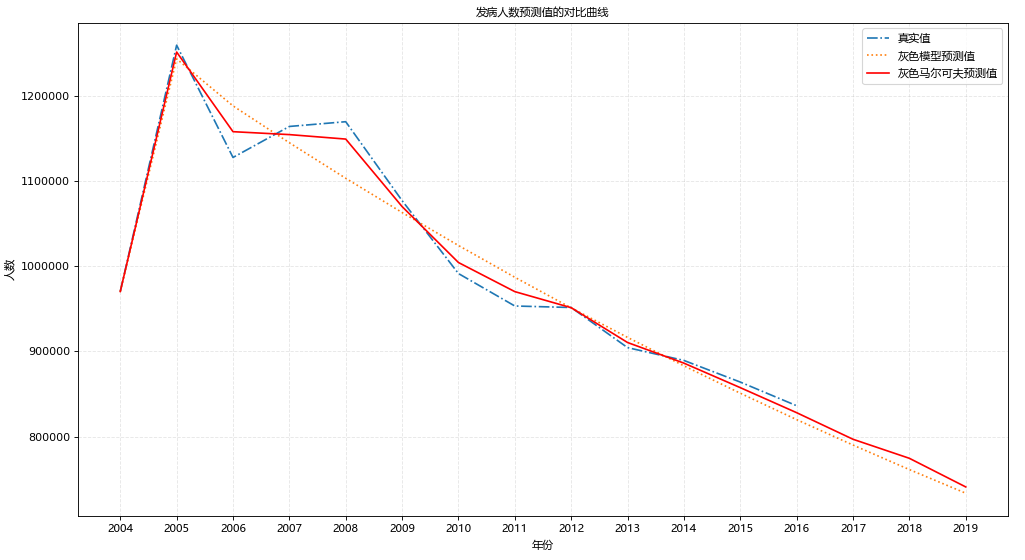
\includegraphics[width=\textwidth]{figures/f.png}
	\caption{发病人数预测对比曲线图}\label{afd}
\end{figure}

	  同理,计算2004-2016年死亡人数预测值得到灰度预测解如下:

	  其误差状态区间如表~\ref{ss}~所示:
	    \begin{table}[H]
	  	\centering\caption{死亡数状态区间划分}\label{ss}
	  	\begin{tabular}{cccc}
	  		\toprule[1.5pt]
	  		\multicolumn{1}{m{2cm}}{\centering 状态}
	  		& \multicolumn{1}{m{3cm}}{\centering $E_{1}$}
	  		& \multicolumn{1}{m{3cm}}{\centering $E_{2}$}
	  		& \multicolumn{1}{m{3cm}}{\centering $E_{3}$}
	  		\\
	  		\midrule[0.5pt]
	  		残差区间 &  $(-684,-228]$  &$(-228,228)$ & $(228,684]$   \\ 
	  		\bottomrule[1.5pt]	
	  	\end{tabular}
	  \end{table}
	  
	  将发病人数预测值归类于误差区间如表~\ref{sss}~所示:
	  \begin{table}[H]
	  	\centering\caption{死亡人数误差状态区间}\label{sss}
	  	\begin{tabular}{cccccccccccccc}
	  		\toprule[1.5pt]
	  		\multicolumn{1}{m{2cm}}{\centering 年份}
	  		& \multicolumn{1}{m{.7cm}}{\centering 2004}
	  		&\multicolumn{1}{m{.7cm}}{\centering 2005}
	  		& \multicolumn{1}{m{.7cm}}{\centering 2006}
	  		& \multicolumn{1}{m{.7cm}}{\centering 2007}
	  		& \multicolumn{1}{m{.7cm}}{\centering 2008}
	  		& \multicolumn{1}{m{.7cm}}{\centering 2009}
	  		& \multicolumn{1}{m{.7cm}}{\centering 2010}
	  		& \multicolumn{1}{m{.7cm}}{\centering 2011}
	  		& \multicolumn{1}{m{.7cm}}{\centering 2012}
	  		& \multicolumn{1}{m{.7cm}}{\centering 2013}
	  		& \multicolumn{1}{m{.7cm}}{\centering 2014}
	  		& \multicolumn{1}{m{.7cm}}{\centering 2015}
	  		& \multicolumn{1}{m{.7cm}}{\centering 2016}
	  		\\
	  		\midrule[0.5pt]
	  		状态区间 &  $E_{2}$  &$E_{2}$ & $E_{2}$&$E_{3}$ &$E_{1}$ &$E_{3}$&$E_{2}$&$E_{2}$&$E_{2}$&$E_{2}$&$E_{1}$&$E_{2}$&$E_{2}$  \\ 
	  		\bottomrule[1.5pt]	
	  	\end{tabular}
	  \end{table}
	   求得初始状态概率向量$t_{0}'$,转移矩阵$P'$为:
	  \begin{gather}
\begin{matrix}
t_{0}'=[2/13,9/13,2/13]\\ 
\\ 
P'=\left(\begin{array}{lll} 0 & 1/2 & 1/2\\ 1/8 & 3/4 & 1/8 \\1/2 & 1/2 & 0\end{array}\right)
\end{matrix}
	  \end{gather}
       得到由灰色预测与马尔科夫校正后预测解如图~\ref{asf}~所示:
     \begin{figure}[H]
	    \centering
     	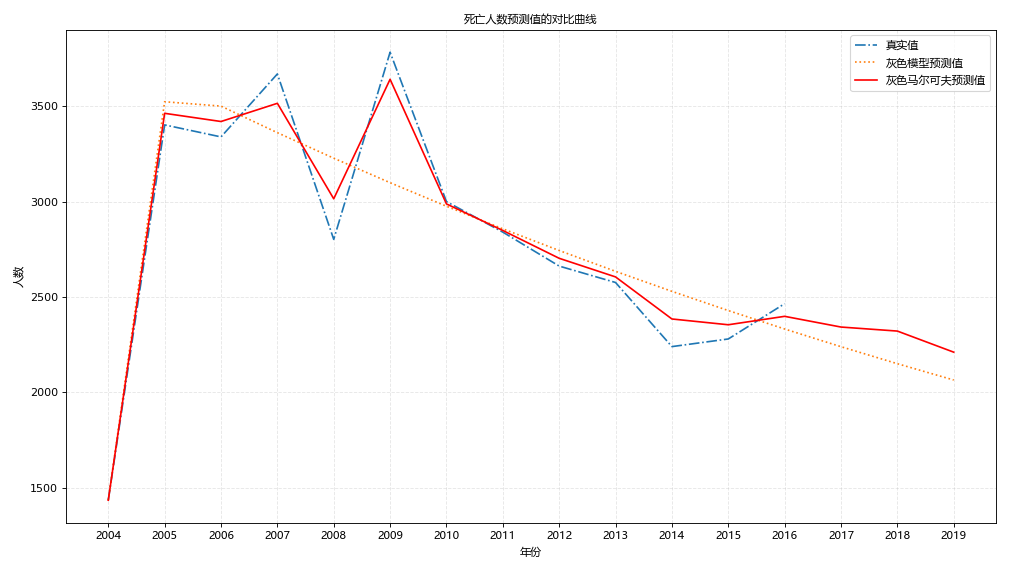
\includegraphics[width=\textwidth]{figures/s.png}
     	\caption{死亡人数预测对比曲线图}\label{asf}
     \end{figure}
 
   \subsection{结果分析}
	由图~\ref{afd}~和图~\ref{asf}~中的预测解曲线直观对比可知,由马尔科夫模型校正后的预测值相较于普通灰色预测值与实际值的拟合度更高,波动性一致,且灰色模型预测值是一条相对平滑的曲线,不能反应实际值的波动。两种模型预测指标如表~\ref{label}~所示:
	
	从上述的预测结果可以得出:利用单独的灰度GM(1,1)模型求出
	的相对误差平均值为xx\%,利用灰色马尔科夫模型修正后求出的相对误差为xx\%,对比原传统灰色模型,降低了误差范围,说明改进后的灰色马尔科夫模型的拟合程度更高,预测效果更好,适用于传染病发病数和死亡数的短期预测。


    
	\section{模型的评价}
	\subsection{模型的优点}
		\begin{itemize}                                             

		\item [(1)] 将多目标优化转换成背包优化问题,自主设计沙石算法,使得船舰的面积利用率高,对船只数量的需求量少。
		\item [(2)] 使用遗传算法,具有很强的全局搜索能力和鲁棒性,运算时间远小于全遍历算法。
	\end{itemize}
	\subsection{模型的缺点}

	遗传算法初始解由卡特蒙洛法随机生成,每次搜索结果不完全相同,可能引起结果的偏差,需要多搜索几次选择才能得到最优结果。
	\subsection{模型改进}
	可使用改进的生命遗传算法,加强算法的局部搜索能力,解决算法早熟的问题。

 
	\newpage	%换页符
	%%参考文献
	%\begin{thebibliography}{9}%宽度9
	% \setlength{\itemsep}{-2mm}
	\nocite{*}		%排版未引用的参考文献
%\bibliography{wenxian.bib}
%	%参考文献添加到wenxian.bib里,再引用
%	
\begin{thebibliography}{9}%宽度9
	\bibitem{bib:one}Saad Ahmed Javed,Sifeng Liu. Correction to: Predicting the research output/growth of selected countries: application of Even GM (1, 1) and NDGM models[J]. Scientometrics,2019,120(3).
	\bibitem{bib:2}李立欣,文海东,许健开.基于灰色马尔可夫模型的能源消耗预测[J].中国科技信息,2018(15):74-75.	
	\bibitem{bib:3}Yawen Wang,Zhongzhou Shen,Yu Jiang. Analyzing maternal mortality rate in rural China by Grey-Markov model[J]. Medicine,2019,98(6).
	\bibitem{bib:4}Saad Ahmed Javed,Sifeng Liu. Correction to: Predicting the research output/growth of selected countries: application of Even GM (1, 1) and NDGM models[J]. Scientometrics,2019,120(3).

\end{thebibliography}

	\newpage
	%附录
	\appendix %%附录

\section{代码}
\subsection{问题一沙石算法--python源代码}
\begin{lstlisting}[language=python]

\end{lstlisting}
\end{document}